\documentclass[12pt, titlepage]{article}

\usepackage{fullpage}
\usepackage[round]{natbib}
\usepackage{multirow}
\usepackage{booktabs}
\usepackage{tabularx}
\usepackage{graphicx}
\usepackage{float}
\usepackage[normalem]{ulem}
\usepackage{hyperref}

\hypersetup{
    colorlinks,
    citecolor=blue,
    filecolor=black,
    linkcolor=red,
    urlcolor=blue
}

%% Comments

\usepackage{color}

\newif\ifcomments\commentstrue %displays comments
%\newif\ifcomments\commentsfalse %so that comments do not display

\ifcomments
\newcommand{\authornote}[3]{\textcolor{#1}{[#3 ---#2]}}
\newcommand{\todo}[1]{\textcolor{red}{[TODO: #1]}}
\else
\newcommand{\authornote}[3]{}
\newcommand{\todo}[1]{}
\fi

\newcommand{\wss}[1]{\authornote{blue}{SS}{#1}} 
\newcommand{\plt}[1]{\authornote{magenta}{TPLT}{#1}} %For explanation of the template
\newcommand{\an}[1]{\authornote{cyan}{Author}{#1}}

%% Common Parts

\newcommand{\progname}{ProgName} % PUT YOUR PROGRAM NAME HERE
\newcommand{\authname}{Team \#, Team Name
\\ Student 1 name
\\ Student 2 name
\\ Student 3 name
\\ Student 4 name} % AUTHOR NAMES                  

\usepackage{hyperref}
    \hypersetup{colorlinks=true, linkcolor=blue, citecolor=blue, filecolor=blue,
                urlcolor=blue, unicode=false}
    \urlstyle{same}
                                


\newcounter{acnum}
\newcommand{\actheacnum}{AC\theacnum}
\newcommand{\acref}[1]{AC\ref{#1}}

\newcounter{ucnum}
\newcommand{\uctheucnum}{UC\theucnum}
\newcommand{\uref}[1]{UC\ref{#1}}

\newcounter{mnum}
\newcommand{\mthemnum}{M\themnum}
\newcommand{\mref}[1]{M\ref{#1}}

\begin{document}

\title{System Design for HairEsthetics}

\author{Team 18 \\ Charlotte Cheng
        \\ Marlon Liu
        \\ Senni Tan
        \\ Qiushi Xu
        \\ Hongwei Niu
        \\ Bill Song
}

\date{\today}

\maketitle

\pagenumbering{roman}

\section{Revision History}

\begin{tabularx}{\textwidth}{p{3cm}p{2cm}X}
\toprule {\bf Date} & {\bf Version} & {\bf Notes}\\
\midrule
Jan 12 & 1.0 & Initial Draft\\
Jan 14 & 1.1 & Minor changes\\
Jan 16 & 1.2 & team review and revision \\
\textcolor{red}{Apr 3} & 2.0 & Revision 1 \\
\textcolor{red}{Apr 4} & 2.1 & Minor update\\
\bottomrule
\end{tabularx}

\newpage

\section{Reference Material}

This section records information for easy reference.

\subsection{\textcolor{red}{Abbreviations and Acronyms}}

\renewcommand{\arraystretch}{1.2}
\begin{tabular}{l l} 
  \toprule		
  \textbf{symbol} & \textbf{description}\\
  \midrule 
  AC & Anticipated Change\\
  AI & Artificial Intelligence \\
  AR & Augumented Reality \\
  API & Application programming interface\\
  App & Application \\
  DAG & Directed Acyclic Graph \\
  M & Module \\
  macOS & Operating system developed by Apple Inc \\
  MG & Module Guide \\
  MIS & Module Interface Specification \\
  ML & Machine Learning \\
  OS & Operating System \\
  R & Requirement\\
  REST & Representational state transfer\\
  RGB & Red, Green, Blue \\
  SC & Scientific Computing \\
  SRS & Software Requirement Specification \\
  UC & Unlikely Change \\
  UI & User Interface\\
  \bottomrule
\end{tabular}

\newpage

\tableofcontents

\newpage

\listoftables

\listoffigures

\newpage

\pagenumbering{arabic}

\section{Introduction}
The purpose of the project is to deliver a comprehensive, well-documented software application that complies with standards set in SRS, HA, VnVPlan, MG, and MIS.
\\
\newline
SRS - \href{https://github.com/marlon4dashen/Hairesthetics/blob/main/docs/SRS/SRS.pdf}{/docs/SRS/SRS.pdf}
\newline
Hazard Analysis - \href{https://github.com/marlon4dashen/Hairesthetics/blob/main/docs/HazardAnalysis/HazardAnalysis.pdf}{/docs/HazardAnalysis/HazardAnalysis.pdf}
\newline
VnVPlan - \href{https://github.com/marlon4dashen/Hairesthetics/blob/main/docs/VnVPlan/VnVPlan.pdf}{/docs/VnVPlan/VnVPlan.pdf}
\newline
MG - \href{https://github.com/marlon4dashen/Hairesthetics/blob/main/docs/Design/SoftArchitecture/MG.pdf}{/docs/SoftArchitecture/MG.pdf}
\newline
MIS - \href{https://github.com/marlon4dashen/Hairesthetics/blob/main/docs/Design/SoftDetailedDes/MIS.pdf}{/docs/SoftDetailedDes/MIS.pdf}


\section{Purpose}
The purpose of this document is to effectively communicate the overall design of a system that complies with SRS's specifications. This includes the choices and considerations made by the development team for the system's constituent parts. By the end of this document, the reader ought to understand in detail:
\begin{itemize}
    \item System-User interactions
    \item Timing constraints that are present with the system design
    \item What is considered as normal operation vs. undesirable events that are likely to occur
    \item Implementation difficulties that may arise as a result of the system design
    \item Individual system components and their functionality
\end{itemize}

\section{Scope}
\noident Many people wonder how a different hairstyle or hair color would look on them in real life. Most of them rely on their imagination and feelings, and some uses some applications with simple filters. Thus, the existing market lacks applications that can accurately simulate their look with a new hairstyle or color.

\subsection{System Context Diagram}
\begin{center}
\begin{figure}[H]
\graphicspath{ {system_context_diagram_1.jpg} }
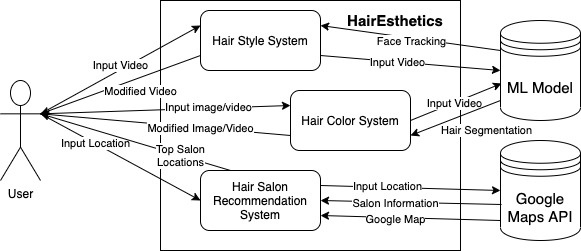
\includegraphics[width=1\textwidth]{system_context_diagram_1}
\caption{System Context Diagram}
\label{Fig_SystemContext} 
\end{figure}
\end{center}

\section{Project Overview}

\subsection{Normal Behaviour}
Under normal conditions, the system shall perform the desired behaviour and produce the desired response. Desired output include transforming image or video with chosen hair color or hairstyle; output recommended hair salon locations and display them on the map. All requirements mentioned in the SRS document will be met.

\subsection{Undesired Event Handling}
Encountering any unexpected events and exceptions during runtime, the system shall pause every operations and present Error screen. The Error screen must inform the user that an undesired event or error have occured and allow the user to redo the last action or re-launch the application. The system will enter the Error screen when one of the following undesired event happened:
\begin{enumerate}
    \item Internet connection lost during salon recommendation operation.
    \item System crash
\end{enumerate}

\subsection{Component Diagram}

\begin{center}
\begin{figure}[H]
% \graphicspath{ {component_diagram.jpg} }
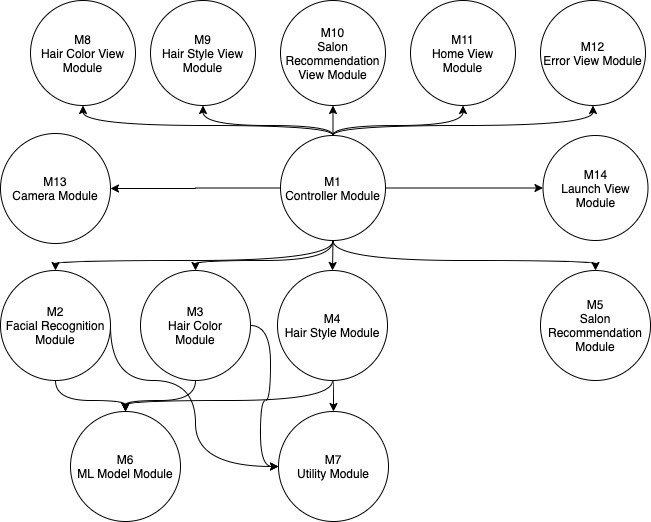
\includegraphics[width=1\textwidth]{Design/SystDesign/component_diagram.jpg}
\caption{Component Diagram Diagram}
\label{Fig_SystemContext} 
\end{figure}
\end{center}

\newpage
\subsection{Connection Between Requirements and Design} \label{SecConnection}

\begin{table}[h]
\caption{Design Decisions} \label{TblDecisions}
\begin{tabularx}{\textwidth}{p{2.5cm}p{6cm}X}
\toprule
\textbf{Requirement Number} & \textbf{Requirement} & \textbf{Design Decision}\\
\midrule
FR1 & The user must input their face in image or video format & Use camera to capture image or video\\
\midrule
FR2 & The system must pre-process the image by transforming the input facial image to grayscale & Use OpenCV library to convert the image to grayscale\\
\midrule
FR3 & The system must perform face shape detection on grayscale facial image & Use OpenCV pre-trained facial detection model to detect face shape\\
\midrule
FR6 & The system must mark the corners and shape with facial landmark coordinates & Use OpenCV facial landmark detection algorithm to mark facial landmarks\\
\midrule
FR7 & The system must store the coordinates from the hair and facial features & Store the coordinates real-time using cache\\
\midrule
HM12 & The system should output the transformed face in image or video & Display the change using the camera view\\
\midrule
HM6 & The system should detect hair edges on detected faces & Use hair segmentation algorithm (UNet) to compute hair edge coordinates\\
\midrule
\sout{LR1} & \sout{The installation process must be completed within 3 steps} & \sout{The app should be available on app store to allow easy installation}\\

\bottomrule
\end{tabularx}
\end{table}
\newpage
\begin{table}[h]
\caption{Design Decisions Continued} \label{TblDecisions}
\begin{tabularx}{\textwidth}{p{2.5cm}p{6cm}X}
\toprule
\textbf{Requirement Number} & \textbf{Requirement} & \textbf{Design Decision}\\
\midrule
ASR1& Fonts shall be in appropriate color and size & Use a predetermined cross-application font family and colors\\
\midrule
SER1 & The application must allow new features to be added in the future &
The application will be designed using a modular architecture\\
\midrule
RER1 & Data from previous builds of the product should be compatible with new builds of the product & Implement version control for data and backwards compatibility for old data\\
\midrule
PRR1 & Users will not be able to access data generated by other users & Do not upload user data to cloud OR use authentication system to prevent malicious users from obtaining data\\

\bottomrule
\end{tabularx}
\end{table}


\section{System Variables}
\subsection{Monitored Variables}
There are no monitored variables for this system

\subsection{Controlled Variables}
There are no controlled variables for this system

\subsection{Constants Variables}
\begin{flushleft}
\begin{table}[H]
\begin{tabularx}{\linewidth}{|l|l|l|X|}
    \toprule {\bf Variable Name} & {\bf Type} & {\bf Value} & {\bf Description}\\
    \midrule
    BROWN & Tuple of Integers & [19, 69, 139] & RGB value\\
    \hline
    PINK & Tuple of Integers & [180, 105, 255] & RGB value\\
    \hline
    WHITE & Tuple of Integers & [255, 255, 255] & RGB value\\
    \hline
    PURPLE & Tuple of Integers & [211, 0, 148] & RGB value\\
    \hline
    GREEN & Tuple of Integers & [113, 179, 60] & RGB value\\
    \hline
    DARKRED & Tuple of Integers & [0, 0, 139]& RGB value\\
    \bottomrule
\end{tabularx}
    \caption{Constants Variables}
\end{table}
\end{flushleft}

\section{User Interfaces}
The user interface for Hairesthetics on MacOS is designed to be intuitive and easy to navigate. The hairstyle simulation view is divided into three main sections: the camera view, the control panel, and the toolbar. The camera view takes up the majority of the screen and allows the user to view and interact with the simulated hair in real-time. The control panel, located on the lower side of the screen, allows the user to adjust various settings, such as hairstyles and hair colors. The toolbar, located at the top of the screen, provides access to common actions such as app settings. \\

\noindent The app settings for Hairesthetics are accessed through a dedicated settings menu, which is accessible from the toolbar. The settings menu allows the user to configure various aspects of the app, including user preferences and app appearance. It also displays details about application version, privacy levels. \\

\noindent The layout and components of the user interface \ref{UI:1} are detailed in the appendix of this document, which was created using Figma, a design tool.

\section{Design of Communication Protocols}

Communication protocols are used to define the rules and procedures for data exchange between different modules or systems. In this project, method invocation is used for communication between modules, which allows one module to call a specific function or method in another module. In addition, REST/HTTPS is used as the communication protocol between the module and external APIs. PythonKit framework is used to allow interaction between Swift and Python. As the Python library are loaded at runtime by PythonKit, it will try to find the most modern Python version available in the system. The PythonKit framework allows calling Python script from Swift.
This allows for seamless integration and communication between the different modules and external systems, ensuring that data is accurately and efficiently exchanged.

\section{Timeline}
This is a rough outline of the timeline for the project, and the specific tasks and their duration may change based on the project's needs.

\begin{table}[H]

\begin{tabularx}{\textwidth}{lXXX}
\toprule
\textbf{Week} & \textbf{Task} & \textbf{Responsible Member(s)}\\
\midrule
1-3 & Facial feature detection and hair segmentation & Marlon Liu, Bill Song \\
& UI/UX design and \sout{ARKit exploration} \textcolor{red}{Three.js simulations} & Charlotte Cheng, Senni Tan \\
\midrule
4-6 & API and model training development & Hongwei Niu \\
& Hair model artist and 3D simulation & Qiushi Xu \\
\midrule
7-8 & Refining and improving computer vision algorithms & Marlon Liu, Bill Song \\
& Implementing AR interface in \sout{iOS} \textcolor{red}{React web} application & Qiushi Xu, Charlotte Cheng, Senni Tan  \\
\midrule
9-10 & Finalizing backend and APIs & Hongwei Niu \\
& Integrating 3D hair simulations into AR interface & Qiushi Xu \\
\midrule
10-13 & Final testing, debugging, and polishing & All Members \\
\bottomrule
\bottomrule
\end{tabularx}
\caption{Timeline} \label{TblTimeline}
\end{table}


% \bibliographystyle {plainnat}
% \bibliography{../../../refs/References}

\newpage{}

\appendix

\section{Interface}

\begin{figure}[H]
  \centering
  \includegraphics[width=0.8\linewidth]{MainView.png}
  \caption{Hairstyle View of the app, exported from Figma}
  \label{UI:1}
\end{figure}
\textcolor{red}{
The AR Hairstyle simulation View of an app allows users to virtually try on different hairstyles in real-time. The interface uses augmented reality (AR) technology to superimpose the selected hairstyle on the user's image or a 3D model of the user's head. The interface has various options for selecting hairstyles, including a sub-menu for dynamically changing hair color. Users will be able to browse through different hairstyles and select the one they want to try on. 
}


\begin{figure}[H]
  \centering
  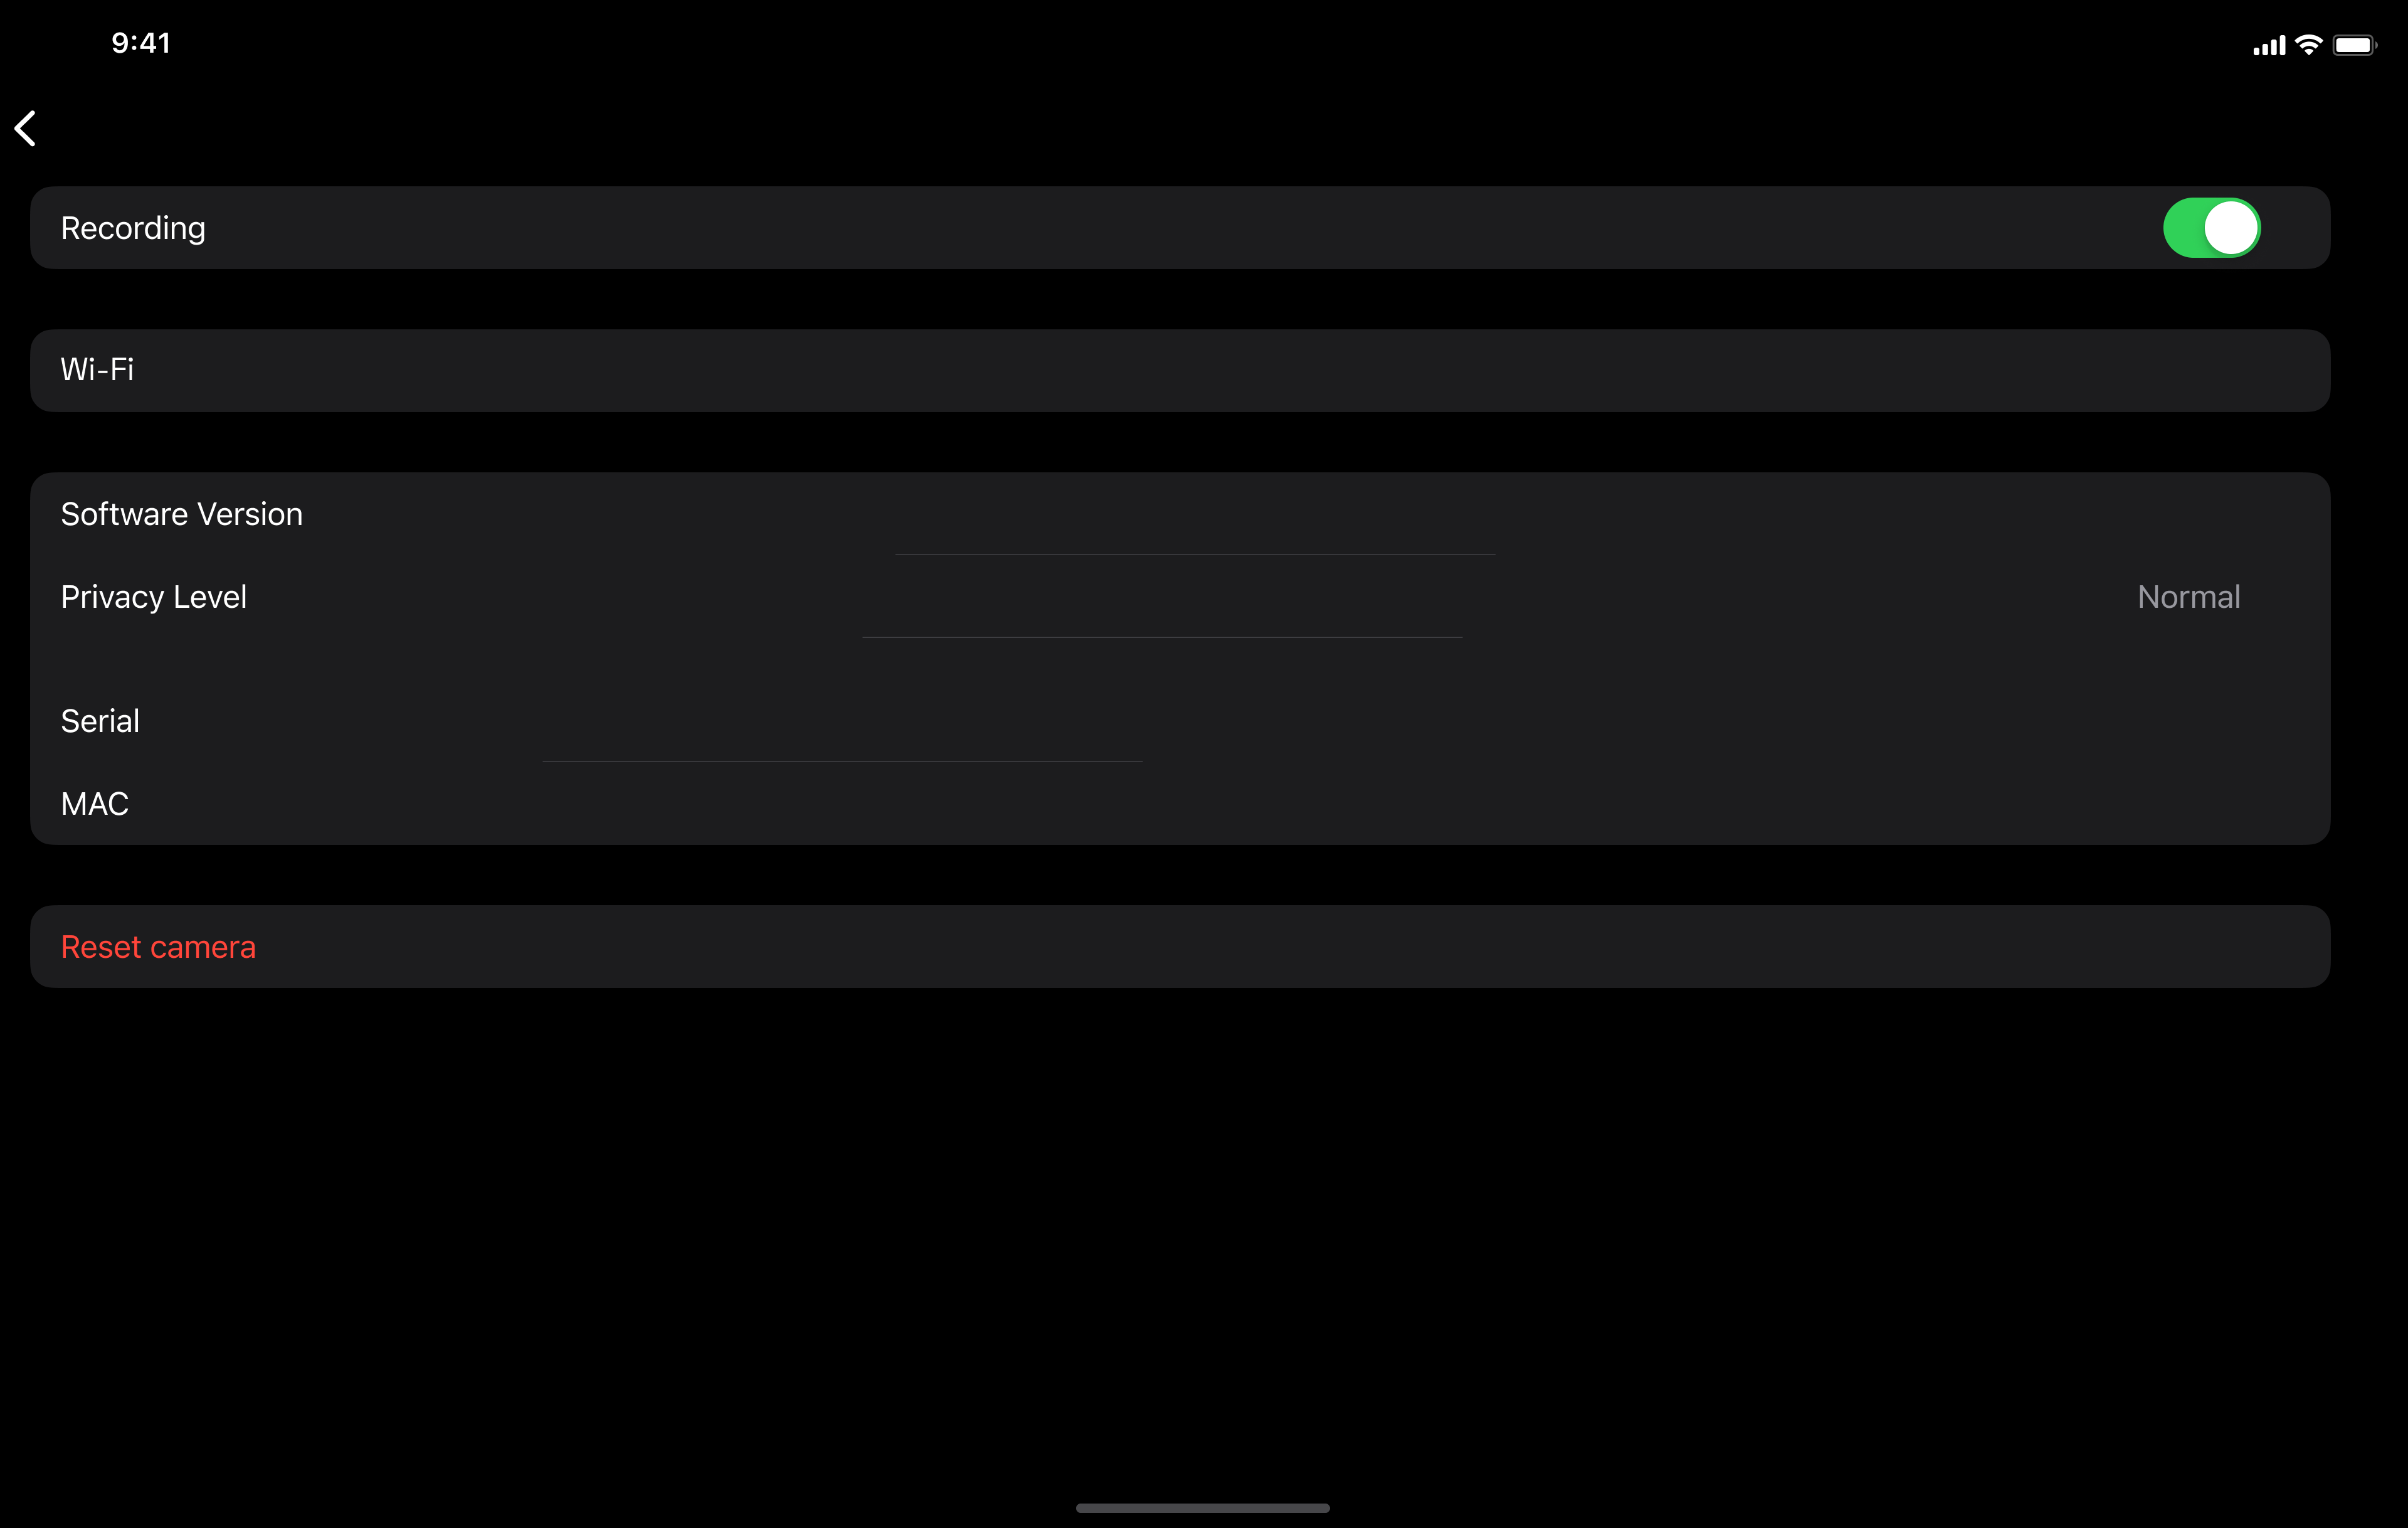
\includegraphics[width=0.8\linewidth]{AppSettings.png}
  \caption{App Settings of the app, exported from Figma}
\end{figure}
\textcolor{red}{
The app settings view allows users to customize and control various aspects of the app. It includes a navigation menu, text fields for software version and buttons for adjusting privacy level, and a help/support section. The settings view is designed to provide users with a personalized app experience that meets their preferences and needs.}

\section{Communication Protocols}

\section{Reflection}

The information in this section will be used to evaluate the team members on the
graduate attribute of Problem Analysis and Design.  Please answer the following questions:

\begin{enumerate}
  \item What are the limitations of your solution?  Put another way, given
  unlimited resources, what could you do to make the project better? (LO\_ProbSolutions)
  \item Give a brief overview of other design solutions you considered.  What
  are the benefits and tradeoffs of those other designs compared with the chosen
  design?  From all the potential options, why did you select documented design?
  (LO\_Explores)
\end{enumerate}

\subsection{Bill Song}
\begin{enumerate}
    \item I am responsible for designing and implementing the facial recognition and hair segmentation system. The current design takes into account of the cost and time constraints. Given with unlimited resources, the ML models can achieve a much better accuracy with much more dataset. Finding high quality training dataset consumes a large amount of time, since our system needs picture of different hair color, angle, and style.
    \item We chose MVC design pattern for designing the hair modification system. It has separate interfaces and models for changing hair color and hair style. I chose this design, because these modules are mostly independent, so they can be implemented, maintained efficiently in parallel. On the UI side, the interface for these systems share some similarities, MVC allows multiple views and avoid code duplication. During the planning phase, I have considered pip-filter architecture, since hair modification system is essentially a data filter and transformation system. This design supports high throughput for excessively data processing but lacks dynamic interactions and configurations. Hairesthetics should provide interesting and engaging interactions with the user.
\end{enumerate}

\subsection{Charlotte Cheng}
\begin{enumerate}
    \item I am responsible for designing the user interface using Figma and implementating it on MacOS using swiftUI. The process of designing the user interface in Figma allowed me to experiment with different layouts and design elements to create a visually appealing and user-friendly interface. However, the transition to implementing the design in SwiftUI was not always smooth. One limitation of my solution for designing the user interface using Figma and implementing it on MacOS using SwiftUI is that it is only compatible with MacOS. Given unlimited resources, I could expand the compatibility of the application to other operating systems such as Windows and Linux, making it more accessible to a wider audience. Additionally, with more resources, I could conduct more extensive user testing to gather valuable feedback and insights to improve the user experience. Furthermore, I could also explore the use of other design tools and technologies to enhance the visual design and functionality of the application, such as incorporating animations and interactive elements.
    \item Another design solution that was considered for this project was implementing the app on iOS. However, this option was not feasible as the PythonKit framework, which is necessary for the integration of Python and Swift, is only compatible with MacOS. One benefit of this design solution is that iOS has a larger user base and more devices available, making the application more accessible to a wider audience. However, the tradeoff is that it would not be able to utilize the PythonKit framework and would require a different method for integration with Python. We eventually decided to go with MacOS app for its compatibility with the PythonKit framework. This allowed for seamless integration with Python and the ability to utilize the full range of functionality provided by the python libraries, which is more important because of the need of Python Machine Learning libraries in the project. 
\end{enumerate}

\subsection{Senni Tan}
\begin{enumerate}
    \item I am responsible for designing and implementing the camera module. The current design is that the camera is controlled by the Swift package called AVFoundation. This package allows the developer to easily start a record session and currently capture inputs from the physical camera component. My design is that then the session will then pass the camera input to the backend. One limitation is that the performance and reliability of this camera component rely on an outer package so we don't have control of it.
    \item Another design solution that we considered is that we can build our own camera component but that is way beyond our experience and knowledge and we may not have time to do this. Also, AVFoundation is a Swift package used by many developers and communities to interact with the backend AR component in their Apps, therefore, this package's performance and reliability are trustable. With all these, we decided to have our design go with using the AVFoundation package.
\end{enumerate}

\subsection{Marlon Liu}
\begin{enumerate}
In summary, I have designed and implemented a facial recognition and hair segmentation system that takes into account cost and time constraints. We have chosen to use the MVC design pattern for our application because it allows for efficient implementation and maintenance of independent modules, it also allows us to follow a test-driven development fashion. I summarized the utility functions into a module to avoid code duplication and apply a better and useful interface in the higher level development. I also designed the hair segmentation module to integrate the result of machine learning model predictions into image masking. During this time, I have learned the mechanics to design a better backend functionalities and utilized them to serve the frontend better. 
\end{enumerate}

\subsection{Qiushi Xu}
\begin{enumerate}
    I am responsible for designing and implementing the hairstyle view module and hair color view module. For now the design can put a AR hair model at a certain coordinate in a certain angle. The future design requires the session pass the camera input to the facial recognition process. Then the hairstyle view module and hair color view would receive the face coordinates to place the ar hair model and color.
    \item Currently one difficulty would be rotate the AR hair model along with the user's face without huge delay. Since running python code in swift has a lag that may cause some delay, we will simplify the coordinates calculation algorithm to reduce the total run time. 
\end{enumerate}

\subsection{Hongwei Niu}
\begin{enumerate}
    Using Python as my primary programming language, I set out to create a solution that would allow users to easily find and choose the perfect salon for their needs. Originally, we chose to use a robust database management system to store and manage the data, instead of using an Excel table and pandas library. A database management system such as MySQL or MongoDB would provide more efficient and reliable data management and handling capabilities. However, we choose not to use database system for outputs for this module and other modules. So the outputs currently stored in a spreadsheet. I began by creating a Python script that utilized the pandas library to read an Excel table containing business information and convert it into a DataFrame. Next, I chose use the Google Maps API to extract additional data such as latitude and longitude of the businesses and add them to the DataFrame. With this data in hand, our group used the SwiftUI library to develop a MacOS application that would allow users to easily view and interact with the information. I think implementing a List view to display the business information from the Core Data entities will be reasonable, then use the Map view to display the location of the businesses on the map by plotting the latitude and longitude obtained from the Google Maps SDK. Additionally, We may use the MapKit framework to interact with the Map view, allowing users to zoom, pan, and explore the map view as needed. In the application UI, we may use the data from the Core Data entities and the additional data from the Google Maps SDK to display the information of the businesses and their locations on the map. Users can search, filter and sort the data to find the perfect salon that fits their needs. 

 
    \item  
\end{enumerate}



\end{document}